%% ------------------------------------------------------------------------- %%
\chapter{Resultados preliminares}
\label{cap:resultados-preliminares}

Este capítulo é parte de um estudo preliminar \citep{marcelo-vem-2019} apresentado no \acrfull{vem} de 2019. Este estudo foi um piloto para avaliar o uso das redes convolucionais no problema de \textit{code retrieval}. Utilizamos as mesmas arquiteturas propostas no capítulo~\ref{cap:abordagem}. E para comparar, utilizamos apenas uma arquitetura de referência \textit{Embedding}.

Os resultados da arquitetura bi-LSTM com CNN e a arquitetura CNN foram promissores. As duas arquiteturas apresentaram um valor da métrica \acrfull{mrr} de $0,60$ e $0,58$ respectivamente. E em $75\%$ das vezes, as respostas corretas apareceram entre as 3 primeiras posições, de um total de 50 possíveis respostas.

\section{Conjunto de dados}
\label{sec:conjunto-dados}

Para este estudo, utilizamos parte do conjunto de dados disponibilizado por \cite{yao-2018}. Este conjunto é formado por $\bm{147.546}$ pares de questões e trechos de código-fonte em Python e $\bm{119.519}$ em SQL. Estes pares foram coletados do site \Gls{sof}. Uma peculiaridade destes dados em relação aos dados utilizados nos outros trabalhos \cite{iyer-etal-2016-summarizing, Allamanis-bimodal-source-code-natural-language:2015}, é o fato de conter questões do tipo \textit{how-to-do-it}. As respostas para este tipo de questão costumam ser mais diretas e ter apenas um trecho de código-fonte como solução \citep{yao-2018}. Estas questões normalmente expressam as intenções do desenvolvedor, indo de encontro com a nossa definição da seção~\ref{sec:code-retrieval-definicao} adotada para o problema de \textit{code retrieval}.

Os dados disponibilizados por \cite{yao-2018} são divididos em 3 (três) subconjuntos distintos. Um subconjunto é formado apenas por questões coletadas do \Gls{sof} que continham apenas um trecho de código-fonte na descrição da resposta. O outro é formado por questões que apresentavam mais de um trecho de código-fonte na descrição. E o terceiro é formado por pares de questões e trechos de código-fonte anotados manualmente.

Nos casos em que há mais de um trecho de código-fonte na descrição da resposta, um trecho de código não é necessariamente uma solução para a pergunta. No exemplo abaixo, os trechos \emph{T2} e \emph{T4} não são soluções para a questão. O trecho \emph{T2} apenas inicializa um array e o trecho \emph{T4} mostra a saída do comando \textit{print} para o vetor já convertido\footnote{Site: \url{https://stackoverflow.com/questions/34349762/convert-2d-numpy-array-to-string} Esta questão apresenta 6 trechos de código-fonte, mas para melhor visualização, optamos por colocar apenas 4 trechos em nosso exemplo\label{foot:exemplo-stackoverflow-mais-de-um-trecho}}.



\begin{tcolorbox}[colframe=orange!75!black,colback=gray!15!white,fonttitle=\bfseries,adjusted title=\large{Título da questão: convert 2d numpy array to string}~\ref{foot:exemplo-stackoverflow-mais-de-um-trecho}]
\begin{mypythongreen}{Trecho T1: A one-liner will do:}
b = '\n'.join('\t'.join('%0.3f' %x for x in y) for y in a)
\end{mypythongreen}

\begin{mypythonred}{Trecho T2: Using a simpler example:}
>>> a = np.arange(25, dtype=float).reshape(5, 5)
>>> a
array([[  0.,   1.,   2.,   3.,   4.],
       [  5.,   6.,   7.,   8.,   9.],
       [ 10.,  11.,  12.,  13.,  14.],
       [ 15.,  16.,  17.,  18.,  19.],
       [ 20.,  21.,  22.,  23.,  24.]])
\end{mypythonred}
\begin{mypythongreen}{Trecho T3: is equivalent to:}
res = []
for y in a:
    res.append('\t'.join('%0.3f' %x for x in y))
b = '\n'.join(res)
\end{mypythongreen}
\begin{mypythonred}{Trecho T4: prints this:}
0.000   1.000   2.000   3.000   4.000
5.000   6.000   7.000   8.000   9.000
10.000  11.000  12.000  13.000  14.000
15.000  16.000  17.000  18.000  19.000
20.000  21.000  22.000  23.000  24.000
\end{mypythonred}
\end{tcolorbox}






Para diferenciar estes casos, \cite{yao-2018} anotaram os pares com $\bm{1}$, quando o trecho é solução para a pergunta e $\bm{0}$, em caso contrário. Esta anotação foi feita automaticamente por um framework proposto no artigo.

Ao final, o conjunto de dados é dividido da seguinte maneira:

\begin{table}[h]
\centering
\begin{tabular}{ p{16em} P{10em} P{10em} }
\hline
  & \multicolumn{2}{c}{\textbf{Questão}}\\
\hline
\textbf{Código-fonte} & \textbf{Python} & \textbf{SQL}  \\
\hline

Apenas 1 trecho de código na descrição da resposta & $85.294$ & $75.637$ \\

Trechos de código-fonte anotados automaticamente & $60.083$ & $41.826$ \\

Trechos de código-fonte anotados manualmente & $2.169$ & $2.056$  \\

 \hline
 \textbf{Total} & $\bm{147.546}$ & $\bm{119.519}$\\
 \hline 
 
\end{tabular}
\caption{Divisão do conjunto de dados disponibilizado por \cite{yao-2018}. O conjunto formado por "Trechos de código-fonte anotados automaticamente" contém questões que tem mais de um trecho de código-fonte por resposta. Quando há mais de um trecho de código-fonte por resposta, nem todo trecho é uma solução. Neste caso, \cite{yao-2018} criaram um framework para anotá-los automaticamente. Eles obtiveram F1 de $0,916$ e acurácia de $0,911$ em seus testes.}
\label{table:summary-training-data-yao-staqc}
\end{table}

\section{Treinamento e avaliação}
\label{sec:treinamento-avaliacao}

Para o treinamento do modelo, utilizamos apenas os pares de questões e trechos de código-fonte em Python. Inicialmente, utilizamos apenas os pares anotados automaticamente. Este conjunto de dados apresenta uma variabilidade maior, em torno de 27\% das questões contém mais de um trecho de código-fonte anotados como correto.

Adotamos o mesmo procedimento de treinamento e avaliação proposto por \cite{iyer-etal-2016-summarizing}. Para o treinamento, foi utilizado o conjunto com $60.083$ pares. Para escolha do modelo e avaliação final foi utilizado o conjunto de dados anotados manualmente.

\begin{table}[h]
\centering
\begin{tabular}{ p{3cm} r  }
 \hline
 \textbf{Amostras} & \textbf{Quantidade de pares $<q_{i}, c_{i}^{+}>$}\\
 \hline
 Treinamento & $60.083$\\
 
 DEV & $1.085$ \\
 
 EVAL & $1.084$\\
 \hline
 \textbf{Total} & $\bm{62.252}$\\
 \hline
\end{tabular}
\caption{Divisão das amostras para treinamento e avaliação. O conjunto de dados é formado por pares $<q_{i}, c_{i}^{+}>$, onde $q_{i}$ é uma questão e $c_{i}^{+}$ é um trecho de código-fonte anotado como correto. O conjunto formado por pares anotados manualmente foi dividido em DEV e EVAL conforme o procedimento descrito por \cite{iyer-etal-2016-summarizing}.}
\label{table:divisao-amostras}
\end{table}

O modelo foi treinado durante 80 épocas. Caso a função de perda \textit{hinge} fique abaixo de $0,001$ o treinamento é interrompido antes. A cada época, o modelo é avaliado na amostra \emph{DEV}. O intuito desta avaliação é obter o melhor modelo conforme a métrica \acrshort{mrr}. Esta avaliação na amostra DEV é feita da seguinte maneira:

Para cada par $<q_{i}, c_{i}^{+}>$ da amostra \emph{DEV}, onde $q_{i}$ uma questão e $c_{i}^{+}$ uma questão anotada como correta. Outros 49 distratores $c'$ são selecionados aleatoriamente da amostra de treinamento, tal que $c_{i}^{+} \neq c'$. Para cada questão, o modelo calcula a similaridade entre a questão e os trechos de código-fonte. O cálculo de similaridade é feito através da função $h_{\theta}$, onde $h_{\theta}$ é a função \textit{cosine}. 

Posteriormente, os trechos de código-fonte são ordenados de forma decrescente, do mais similar (maior pontuação) ao menos similar (menor pontuação). Com os trechos ordenados, obtém-se a posição do trecho $c_{i}^{+}$ para cálculo do \textit{reciprocal rank}. \textit{Reciprocal rank} é o inverso da posição da primeira ocorrência de $c_{i}^{+}$ encontrada no resultado. Com o \textit{reciprocal rank}, calcula-se o \acrshort{mrr} para a amostra. \acrshort{mrr} pode ser definido como \citep{Gu-deep-code-search:2018}:

\begin{equation}
MRR = \frac{1}{n} * \sum_{i = 1}^{n}\frac{1}{p_{i}^{+}}    
\end{equation}



Onde $n$ é a quantidade de questões presentes na amostra, $p_{i}^{+}$ é a posição da primeira ocorrência do trecho $c_{i}^{+}$ entre os trechos ordenados.

Este procedimento é repetido durante 20 vezes. A cada iteração, outros 49 distratores são selecionados. Ao final, obtém-se a média \emph{MRR} do modelo.

O modelo que obtiver a maior média \emph{MRR} ao final do treinamento (após 80 épocas ou função de perda menor que $0,001$) é escolhido.

A avaliação final na amostra \emph{EVAL} utiliza o mesmo procedimento da amostra \emph{DEV} descrito acima.

\section{Pré-processamento}

Diferente do trabalho de \cite{tan-lstm-qa}, nós geramos duas matrizes de representação distribuída distintas $\bm{T_{q}}$ e $\bm{T_{c}}$ para o vocabulário das questões e para o vocabulário dos trechos de código-fonte, conforme citado no capítulo~\ref{cap:abordagem}.

Antes de gerar a matriz $\bm{T_{c}}$, utilizamos uma função disponibilizada por \cite{yao-2018} para fazer um pré-processamento dos trechos de código-fonte. Esta função substitui os valores literais numéricos e textos pelas palavras \emph{"NUMBER"} e \emph{"SRING"}. Além disso, os comentários são removidos e as variáveis são substituídas por \emph{"VAR"}. E o caractere de quebra de linha é substituído por \emph{"NEWLINE"}.

As matrizes $\bm{T_{q}}$ e $\bm{T_{c}}$ são geradas pelo \textit{word2vec} com \textit{skip-gram}. Na figura~\ref{fig:tsne-code-snippet-python} abaixo, podemos visualizar um exemplo da representação do vetor de representação distribuída gerada pelo \textit{word2vec}. Esta imagem foi criada com o auxílio da ferramenta \textit{t-SNE}. Ela auxilia na visualização de dados de dimensão elevada \citep{scikit-learn-tsne-2019, quora-tsne-2019}.

De acordo com a figura~\ref{fig:tsne-code-snippet-python}, as palavras \emph{from} e \emph{import} são similares. Assim como \emph{if} e \emph{else}, e também \emph{list}, \emph{dict} e \emph{set}, por exemplo.

\begin{figure}[h]
\includegraphics[width=1\textwidth]{figuras/cap-resultados-preliminares/code-tsne-output.png}
\caption{Representação em 2D do vetor de representação distribuída de trechos de código-fonte. Imagem gerada através da ferramenta t-SNE. E o vetor de representação distribuída foi criado a partir da amostra de trechos de código-fonte em Python disponibilizada por \cite{yao-2018}. Vetor criado utilizando o \textit{word2vec} com o algoritmo \textit{skip-gram} e o parâmetro \textit{window} com o valor $5$.}
\label{fig:tsne-code-snippet-python}
\end{figure}

\section{Arquiteturas}

Para este estudo, comparamos as arquiteturas bi-LSTM com CNN e CNN com uma arquitetura de referência \textit{Embedding}. A arquitetura \textit{Embedding} combina os vetores de representação distribuída de cada palavra através de uma camada \textit{max pool}. As outras arquiteturas seguem a descrição feita no capítulo~\ref{cap:abordagem}.

A figura~\ref{fig:arquitetura-bi-lstm-com-cnn}, figura~\ref{fig:arquitetura-cnn} e a figura~\ref{fig:arquitetura-embedding} ilustram as arquiteturas utilizadas:

\begin{figure}[h]
    \centering
    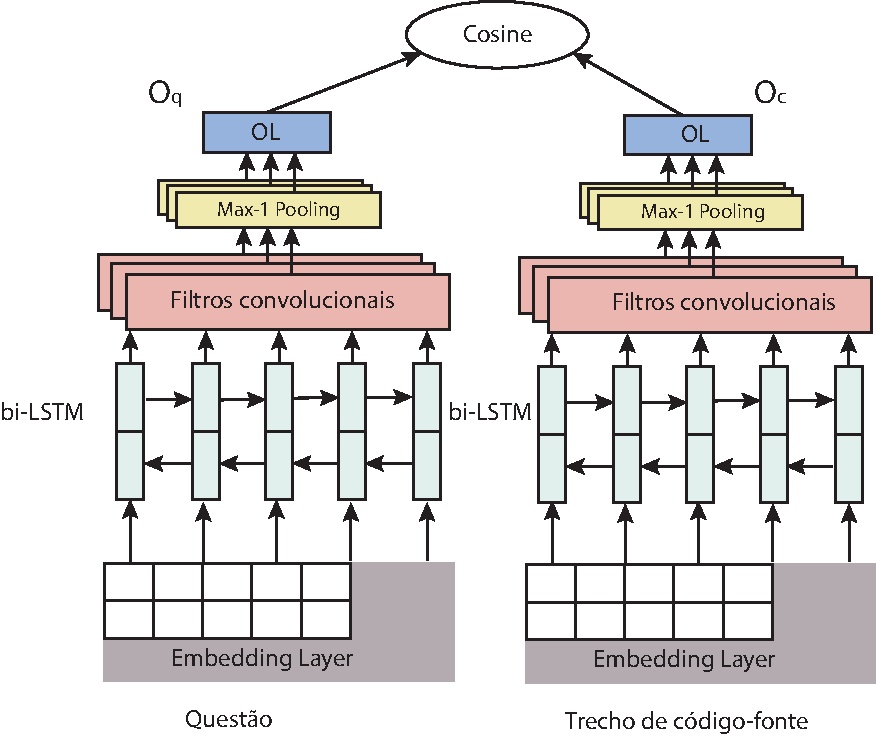
\includegraphics[width=0.6\textwidth]{figuras/cap-resultados-preliminares/ArquiteturaBiLSTM.pdf}
    \caption{Figura da arquitetura bi-LSTM com CNN proposta para o problema do \textit{code retrieval}. Descrição detalhada da arquitetura na seção~\ref{sec:representation-bi-lstm-cnn}. Figura utilizada no artigo \cite{marcelo-vem-2019}}
    \label{fig:arquitetura-bi-lstm-com-cnn}
\end{figure}

\begin{figure}[h]
    \centering
    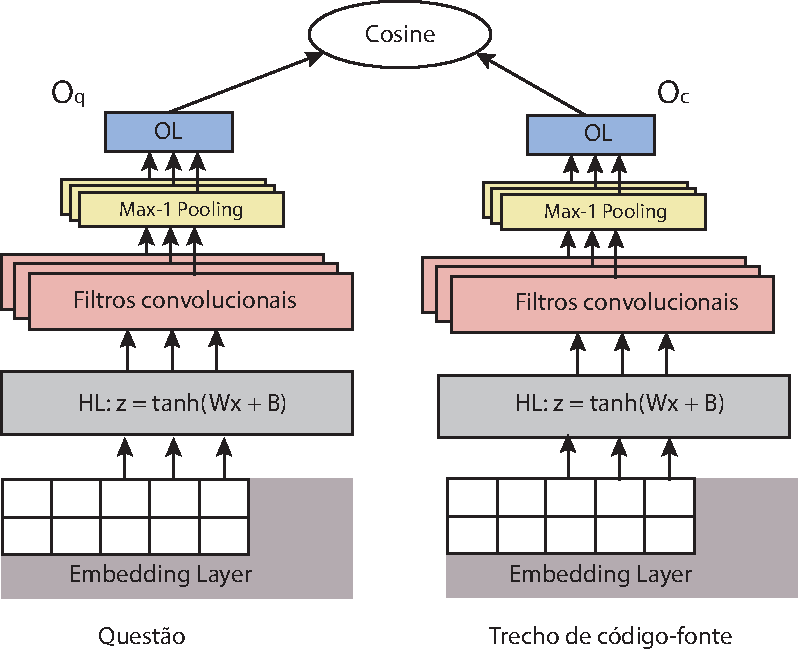
\includegraphics[width=0.6\textwidth]{figuras/cap-resultados-preliminares/ArquiteturaCNN.pdf}
    \caption{Figura da arquitetura CNN com a primeira camada de \textit{hidden layer} proposta para o problema do \textit{code retrieval}. Descrição detalhada da arquitetura na seção~\ref{sec:representation-cnn}. Figura utilizada no artigo \cite{marcelo-vem-2019}}
    \label{fig:arquitetura-cnn}
\end{figure}

\begin{figure}[h]
    \centering
    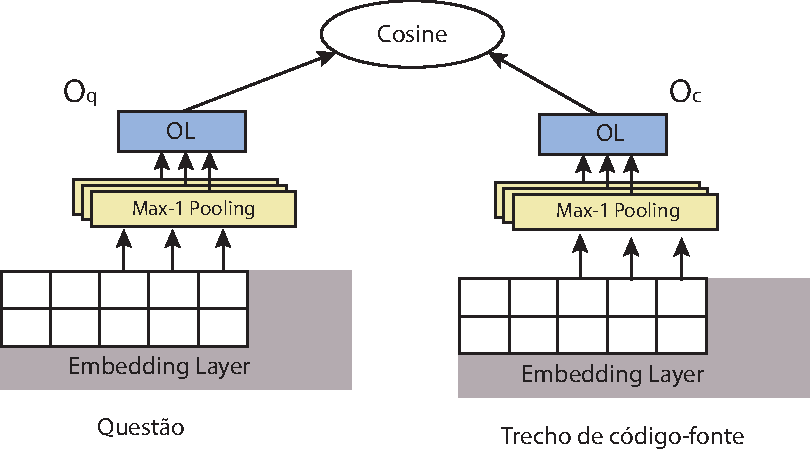
\includegraphics[width=0.6\textwidth]{figuras/cap-resultados-preliminares/ArquiteturaEmbedding.pdf}
    \caption{Figura da arquitetura de referência \textit{Embedding} para comparação. Figura utilizada no artigo \cite{marcelo-vem-2019}}
    \label{fig:arquitetura-embedding}
\end{figure}
Nas figuras \ref{fig:arquitetura-bi-lstm-com-cnn}, \ref{fig:arquitetura-cnn} e \ref{fig:arquitetura-cnn}, a palavra \textit{Embedding Layer} refere-se ao vetor de representação distribuída das palavras. \emph{OL} é um acrônimo de \textit{Output Layer} ou camada de saída. $O_{q}$ indica a camada de saída da questão. $O_{c}$ indica a camada de saída do trecho de código-fonte.

Todas as arquiteturas utilizam uma camada \textit{max pool} e, ao final, calculam a similaridade atravás da função \textit{cosine}.
Não realizamos otimização ou ajustes dos hiper-parâmetros dos modelos. Utilizamos os mesmos hiper-parâmetros propostos por \cite{tan-lstm-qa}. Exceto o hiper-parâmetro filtro da camada CNN, neste caso utilizamos o valor $100$, pois o valor $1000$ proposto por \cite{tan-lstm-qa} aumentou a capacidade do modelo e estava causando \textit{overfitting}.

Para a função de perda \textit{hinge}, utilizamos o valor $0,009$ proposto por \cite{feng-2015} para a margem. Em relação a dimensão do vetor de representação distribuída das palavras (\textit{word embedding}), utilizamos o valor $100$.


%% ------------------------------------------------------------------------- %%
\section{Resultados preliminares}

Os resultados preliminares foram coletados a partir da avaliação dos modelos na amostra \emph{EVAL}. O valor final MRR é a média obtida após 20 iterações. 

\begin{table}[h]
\centering
\begin{tabular}{ p{3cm} P{5cm} }
 \hline
 \textbf{Modelos} & \textbf{Resultados (MRR)}\\
 \hline
 Embedding & $0,52 \pm 0,01$\\
 
 CNN & $0,58 \pm 0,01 $ \\
 
 \textbf{bi-LSTM-CNN} & $\bm{0,60} \pm \bm{0,02}$\\
 \hline
\end{tabular}
\caption{Resultado preliminar do modelo bi-LSTM-CNN proposto em comparação a outros dois modelos (CNN e Embedding). Estes resultados foram obtidos a partir da amostra EVAL.}
\label{table:resultados-preliminares}
\end{table}

Conforme a tabela~\ref{table:resultados-preliminares}, tanto o \emph{CNN} quanto o bi-LSTM com CNN obtiveram resultados próximos. O\emph{CNN} obteve um resultado relativamente menor, mas o seu tempo de duração de treinamento é de apenas 6s. Enquanto o treinamento do bi-LSTM durou cerca de 48 minutos. Tanto o treinamento quanto a avaliação foram executadas na plataforma \Gls{colab} do Google. No momento de treinamento e coleta dos resultados, a execução foi feita em uma máquina virtual com acesso a uma \acrshort{vgpu} Tesla K80.

Para entender um pouco melhor o resultado da média harmônica MRR, a figura abaixo exibe as posições da primeira ocorrência do trecho de código-fonte encontradas durante a avaliação dos modelos.

\begin{figure}[h]
    \centering
    \includegraphics[width=1\textwidth]{figuras/cap-resultados-preliminares/histogram_results.png}
    \caption{Figura das primeiras posições observadas para o trecho de código-fonte anotado como correto.}
    \label{fig:histogram-mrr}
\end{figure}


Tanto o bi-LSTM com CNN quanto CNN conseguiram classificar os trechos de código-fonte entre as 3 (três) primeiras posições em 75\% dos casos. O modelo bi-LSTM com CNN obteve uma precisão TOP-1 de 51\%, i.e., em mais da metade das vezes, o trecho de código-fonte relevante ficou na primeira posição. 

No exemplo abaixo\footnote{Este exemplo refere-se a questão \url{https://stackoverflow.com/questions/24593478/python-and-appending-items-to-text-and-excel-file}\label{foot:exemplo-resultados-preliminares}}, a rede bi-LSTM com CNN conseguiu mostrar o trecho de código-fonte anotado como correto na primeira posição.
No caso do CNN, apesar de não apresentar o trecho propriamente anotado, ele apresentou outro trecho que também serve como resposta. Neste caso, apesar de ter sido penalizado, ele conseguiu responder a questão. 

\begin{tcolorbox}[colframe=orange!75!black,colback=gray!15!white,fonttitle=\bfseries,adjusted title=\large{Python and appending items to text and \colorbox{green}{excel} \colorbox{green}{file}}~\ref{foot:exemplo-resultados-preliminares},
enlarge top by=1cm%equivalent to mdframed 'skipabove'
]
\begin{mypython-without-margin}{bi-LSTM com CNN}
Yvalues = [1, 2, 3, 4, 5]
file_out = |\colorbox{green}{open}|('file.csv','wb')
mywriter=|\colorbox{green}{csv}|.|\colorbox{green}{writer}|(file_out, delimiter = '\n')
mywriter.|\colorbox{green}{writerow}|(Yvalues)
file_out.close()
\end{mypython-without-margin}

\begin{mypython-without-margin}{CNN}
import csv

with |\colorbox{green}{open}|("output.csv", "wb") as f:
    writer = |\colorbox{green}{cwv}|.|\colorbox{green}{writer}|(f)
    writer.|\colorbox{green}{writerows}|(a)
\end{mypython-without-margin}

\end{tcolorbox}

\subsection{Ameaças à validade}

Conforme citado anteriormente, \cite{yao-2018} anotou o conjunto de dados utilizando um framework proposto em seu artigo. Para anotá-los, ela treinou uma rede neural no conjunto de dados anotado manualmente. Em nosso trabalho, fizemos o caminho oposto. Treinamos os nossos modelos nos dados anotados automaticamente e avaliamos no conjunto anotado manualmente. Para diminuir o viés, adotamos o procedimento proposto por Iyer descrito na seção~\ref{sec:treinamento-avaliacao}.

\subsection{Considerações}

Os resultados apresentados pelo modelo bi-LSTM com CNN e CNN parecem bastante promissores, a nosso ver. O próximo passo é comparar os nossos modelos com o modelo proposto por \cite{Sachdev-neural-code-search:2018} que é o estado da arte. 

Tanto o bi-LSTM com CNN e CNN tem uma margem a melhorar. Não fizemos ajustes dos hiper-parâmetros e nem uso de regularização durante o treinamento.

Nas figuras \ref{fig:grafico-erro-bi-lstm-cnn}, \ref{fig:grafico-erro-cnn} e \ref{fig:grafico-embedding} abaixo, podemos ver que tanto bi-LSTM com CNN quanto o CNN apresentam uma diferença grande entre o erro na amostra de validação e o erro na amostra de treinamento. Um indicativo de \textit{overfitting}. Já a arquitetura \textit{Embedding} apresentou um erro de generalização próxima a do treinamento. 

\begin{figure}[h]
    \centering
    \includegraphics[width=1\textwidth]{figuras/cap-resultados-preliminares/569229_ConvolutionalLSTM_plot.png}
    \caption{Gráfico do treinamento do modelo bi-LSTM com CNN. Gráfico do erro de generalização (\emph{val\_loss}) e erro na amostra de treinamento (\emph{loss}) por época (\emph{eixo X}). O melhor modelo em relação a métrica MRR foi obtido na época $9$.}
    \label{fig:grafico-erro-bi-lstm-cnn}
\end{figure}

\begin{figure}[h]
    \centering
    \includegraphics[width=1\textwidth]{figuras/cap-resultados-preliminares/569229_ConvolutionModel_plot.png}
    \caption{Gráfico do treinamento do CNN. Gráfico do erro de generalização (\emph{val\_loss}) e erro na amostra de treinamento (\emph{loss}) por época (\emph{eixo X}). O melhor modelo em relação a métrica MRR foi obtido na época $9$.}
    \label{fig:grafico-erro-cnn}
\end{figure}

\begin{figure}[h]
    \centering
    \includegraphics[width=1\textwidth]{figuras/cap-resultados-preliminares/569229_EmbeddingModel_plot.png}
    \caption{Gráfico do treinamento do modelo \textit{Embedding}. Gráfico do erro de generalização (\emph{val\_loss}) e erro na amostra de treinamento (\emph{loss}) por época (\emph{eixo X}). O melhor modelo em relação a métrica MRR foi obtido na época $39$.}
    \label{fig:grafico-embedding}
\end{figure}

Além da margem de melhora no treinamento, uma análise mais detalhada do resultado é necessário. Conforme o exemplo citado na seção anterior, o modelo CNN apresentou uma resposta correta para a pergunta, porém foi penalizada pois não era exatamente o trecho anotado como correto. 

Caso haja mais casos deste tipo, podemos adotar o mesmo procedimento proposto por \cite{Sachdev-neural-code-search:2018} de avaliação automática. Um trecho será considerado correto quando a diferença entre ele e o trecho anotado como correto for menor que um certo valor.
